\documentclass[../main.tex]{subfiles} % required, if the Chapter be a seperate doc

\begin{document}

\chapter{Statistik}\label{ch:statistik}

\begin{itemize}
    \item \textmathbar{x} - Arithmetischer Mittelwert
    \item $\Delta$h - länge der gespanten Feder vom start der Messung Ohne belastung
    \item s - Standartabweichung des Einzelwertes
    \item $\Delta$\textmathbar{x} - Standartabweichtung des Mittelwertes
    \item r - Relativer Fehler
    \item D - Federkonstante
    \item R\textsuperscript{2} - Korrelationskoeffizient
\end{itemize}

\section{Kraft berechnung}\label{sec:force-calculation}

Die Kraft wurde mit der Newtonischen Formel berechnet

$$ F = m * a $$

$a$ ist in diesem fall die Gravitation der Erde: 9.81 m/s\textsuperscript{2}

\begin{center}
    \begin{tabular}{ |l|l| } \hline\rowcolor{Gray!50}
        Masse [g] & Kraft [N] \\\hline
        0.00      & 0.0000    \\\hline
        0.01      & 0.0981    \\\hline
        0.02      & 0.1961    \\\hline
        0.03      & 0.2942    \\\hline
        0.04      & 0.3923    \\\hline
        0.05      & 0.4903    \\\hline
        0.10      & 0.9807    \\\hline
        0.15      & 1.4710    \\\hline
        0.20      & 1.9613    \\\hline
    \end{tabular}
\end{center}

\section{Feder 1}\label{sec:feder-12}

\begin{center}
    \begin{tabular}{ |l|l|l|l|l|l| }\hline\rowcolor{Gray!50}
        Index & \textmathbar{x} [cm]  & $\Delta$h [cm]        & s [cm]   & $\Delta$\textmathbar{x} [cm] & r [\%]  \\\toprule\hline
        0     & 74.300                & 0.000                 & 0.000000 & 0.000                        & 0.00000 \\\hline
        1     & 73.43\textoverline{3} & 0.86\textoverline{6}  & 0.057735 & 0.03\textoverline{3}         & 0.57735 \\\hline
        2     & 72.63\textoverline{3} & 1.66\textoverline{6}  & 0.057735 & 0.03\textoverline{3}         & 0.57735 \\\hline
        3     & 71.800                & 2.500                 & 0.000000 & 0.000                        & 0.00000 \\\hline
        4     & 71.03\textoverline{3} & 3.26\textoverline{6}  & 0.057735 & 0.03\textoverline{3}         & 0.57735 \\\hline
        5     & 70.16\textoverline{6} & 4.13\textoverline{3}  & 0.057735 & 0.03\textoverline{3}         & 0.57735 \\\hline
        6     & 66.13\textoverline{3} & 8.16\textoverline{6}  & 0.057735 & 0.03\textoverline{3}         & 0.57735 \\\hline
        7     & 62.03\textoverline{3} & 12.26\textoverline{6} & 0.057735 & 0.03\textoverline{3}         & 0.57735 \\\hline
        8     & 58.050                & 16.250                & 0.050000 & 0.028868                     & 0.57735 \\\hline
    \end{tabular}
\end{center}
\begin{figure}[h]
    \centering
    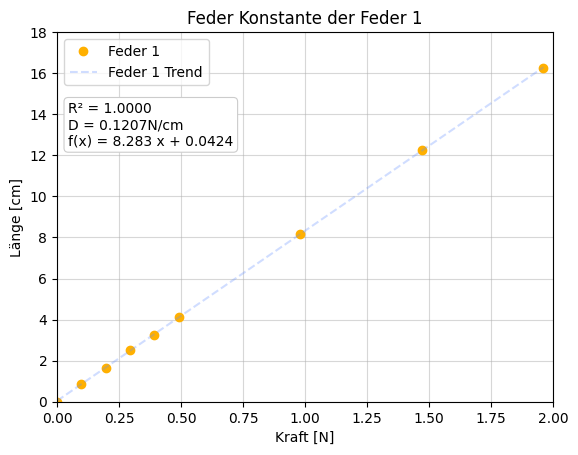
\includegraphics[scale=0.8]{graph/Spring-1}
    \caption{Graph von den gemessenen Werte von Feder 1 dargestellt und darstellung der Trendline}
    \label{fig:graph-spring-1}
\end{figure}
\begin{center}
    \begin{tabular}{ |l|r| } \hline
        Arithmetischer wert von \textmathbar{x}                             & 68.8426 cm            \\\hline
        Arithmetischer wert von s                                           & 0.0440 cm             \\\hline
        Arithmetischer wert von $\Delta$\textmathbar{x}                     & 0.0254 cm             \\\hline
        s des Mittelwertes von Mittelwert von s                             & 0.0147 cm             \\\hline
        Relativer Fehler von s Mittelert und Mittelwert von \textmathbar{x} & 0.0213 cm             \\\hline
        Streuung der Messwerte                                              & x = (x $\pm$ 0.04) cm \\\hline
        R\textsuperscript{2}                                                & 1.0000                \\\hline
        D                                                                   & 0.1207 N/cm           \\\hline
        f(x)                                                                & 8.283x + 0.0424       \\\hline
    \end{tabular}
\end{center}

\section{Feder 2}\label{sec:feder-22}

\begin{center}
    \begin{tabular}{ |l|l|l|l|l|l| }\hline\rowcolor{Gray!50}
        Index & \textmathbar{x} [cm]  & $\Delta$h [cm]        & s [cm]   & $\Delta$\textmathbar{x} [cm] & r [\%]  \\\toprule\hline
        0     & 74.11\textoverline{6} & 0.000                 & 0.000000 & 0.000                        & 0.00000 \\\hline
        1     & 73.300                & 0.86\textoverline{6}  & 0.057735 & 0.03\textoverline{3}         & 0.57735 \\\hline
        2     & 72.53\textoverline{3} & 1.58\textoverline{3}  & 0.057735 & 0.03\textoverline{3}         & 0.57735 \\\hline
        3     & 71.71\textoverline{6} & 2.400                 & 0.000000 & 0.000                        & 0.00000 \\\hline
        4     & 71.91\textoverline{6} & 3.200                 & 0.057735 & 0.03\textoverline{3}         & 0.57735 \\\hline
        5     & 70.100                & 4.01\textoverline{6}  & 0.057735 & 0.03\textoverline{3}         & 0.57735 \\\hline
        6     & 66.000                & 8.11\textoverline{6}  & 0.057735 & 0.03\textoverline{3}         & 0.57735 \\\hline
        7     & 61.96\textoverline{6} & 12.150                 & 0.057735 & 0.03\textoverline{3}         & 0.57735 \\\hline
        8     & 57.900                & 16.21\textoverline{6} & 0.050000 & 0.028868                     & 0.57735 \\\hline
    \end{tabular}
\end{center}

\section{Seriell}\label{sec:seriell2}

\section{Parallel}\label{sec:parallel2}

\end{document}